\scanpage{16}
\figure{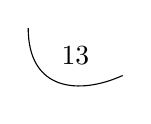
\begin{tikzpicture}[x=1cm,y=1cm]
\node at (0,0) {\mspage{13}};
\draw (-.6,.35) .. controls (-.6,-.45) and (.05,-.5) .. (.6,-.25);
\end{tikzpicture}}
sending $\mathbf L_0$ to $L$, \inserted{\figure{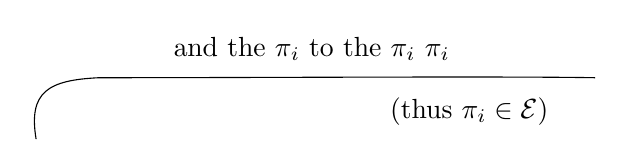
\begin{tikzpicture}[x=1cm,y=1cm]\node at (0,.6) {and the $\boldsymbol\pi_i$ to the $\pi_i$ \deleted{$\unsure{\pi_i}$}};\node at (2,-.2) {(thus $\pi_i\in\mathcal E$)};\draw (-3.5,-.55) .. controls (-3.6,.05) and (-3.35,.2) .. (-2.7,.23) .. controls (-.6,.23) and (2.4,.25) .. (3.6,.23);\end{tikzpicture}}}.
\deleted{\unsure{expressing|respecting} the grading of $\mathcal E$ by $(1.3)$}.
\margin{\figure{
\begin{tikzpicture}
\node[align=center] at (0,0) {essential\\condition !};
\draw (0,0) ellipse (1.65cm and .9cm);
\draw (-1,.6)--(.1,.7);
\end{tikzpicture}}}

Moreover, under these conditions, the homomorphism announced \deleted{\unsure{some}} in (ii) is unique, and with the notation of n\textsuperscript{o} 6, it sends $\unsure{\boldsymbol\Lambda_0|\boldsymbol\Lambda}$ to $\Lambda$, the \deleted{$\unsure{\pi_{i\alpha}}$} $\boldsymbol\pi_{i\alpha}$ to $\pi_{i\alpha}$, $\boldsymbol\pi_i$ to $\pi_i$, $\boldsymbol\varphi_i^{\beta,\alpha}$ to $\varphi_i^{\beta,\alpha}$ \deleted{$\unsure{\varphi_{i,\alpha}^{j,\beta}}$}.
\margin{\figure{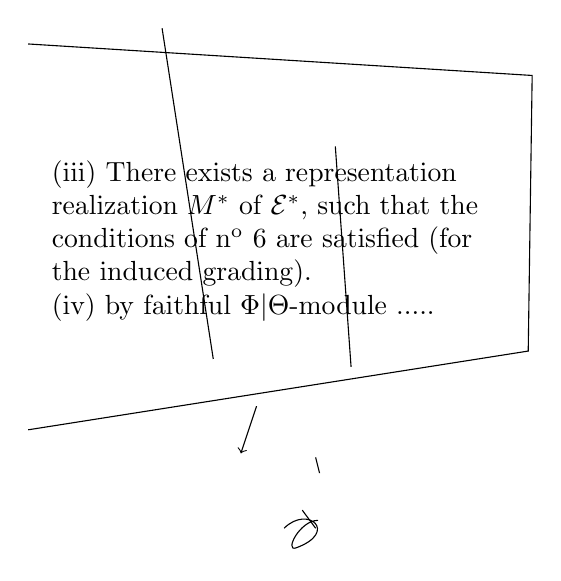
\begin{tikzpicture}
\node[align=left,text width=5.8cm] at (0,0) {\unsure{(iii) There exists a \deleted{representation} \uline{realization} $M^*$ of $\mathcal E^*$, such that the conditions of n\textsuperscript{o} 6 are satisfied (for the induced grading).\\(iv) by faithful $\uline{\unsure{\Phi|\Theta}}$-module .....}};
\draw (-3.2,2.5)--(3.2,2.1)--(3.15,-1.4)--(-3.2,-2.4);
\draw (-1.5,2.7)--(-.85,-1.5);
\draw[thin] (.7,1.2)--(.9,-1.6);
\draw[->] (-.3,-2.1)--(-.5,-2.7);
\draw (.45,-2.75)--(.5,-2.95);
\draw (.05,-3.65) .. controls (.35,-3.35) and (.75,-3.7) .. (.2,-3.9) .. controls (.05,-3.95) and (.25,-3.55) .. (.48,-3.55);
\draw (.28,-3.42)--(.45,-3.65);
\end{tikzpicture}}}

\uline{Proof} $(i)\Rightarrow(ii)$ Follows from the multiplication table of the $\varphi_i^{\beta,\alpha}$ given in n\textsuperscript{o} 6, and from the theorem given in n\textsuperscript{o} 6.

$(ii)\Rightarrow(i)$ \deleted{Let $\pi'_i$ be the images of the $\boldsymbol\pi_i$. We have
\[
\text{with}\qquad L^\alpha\pi'_i=\pi'_{i+\alpha}L^\alpha
\]
thus see that the $\pi'_i$ define the grading of $\mathcal E$, because they are of degree $0$.
I say that $\pi'_i=\pi_i$ for all $i$. Cf Proposition below for this point, applied to $\Phi\longrightarrow\operatorname{End}(M^*)$.}

Since we have, for all $i\leq n$
\[
(\boldsymbol\Lambda_0^{n-i}\mathbf L_0^{n-i}-1)\boldsymbol\pi_i=0,\qquad
(\mathbf L_0^{n-i}\boldsymbol\Lambda_0^{n-i}-1)\boldsymbol\pi_{2n-i}=0
\]
we conclude from this, applying $\varphi$ (and setting $\Lambda'=\varphi(\boldsymbol\Lambda)$)
\[
(\Lambda'^{n-i}L^{n-i}-1)\pi_i=0,\qquad(L^{n-i}\Lambda'^{n-i}-1)\pi_{2n-i}=0.
\]
Thus condition (ii) of the theorem of n\textsuperscript{o} 6 is satisfied, thus also condition (i).

For the uniqueness of $\varphi$, \deleted{\unsure{and the properties}}\inserted{it suffices} \deleted{\unsure{and the relations}} to see that $\varphi(\boldsymbol\Lambda)=\Lambda$, and \inserted{for $\varphi(\boldsymbol\pi_{i,\alpha})=\pi_{i,\alpha}$,} \deleted{\unsure{for this}} \deleted{For $\begin{gathered}\varphi(\boldsymbol\Lambda\\\unsure{\pi_{i,\alpha}}\end{gathered}$} taking into account $\varphi(\boldsymbol\pi_i)=\pi_i$, \deleted{\unsure{thus we have}} the \inserted{\figure{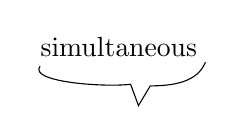
\begin{tikzpicture}[x=1cm,y=1cm]
\node at (0,.4) {simultaneous};
\draw (-1,.15) .. controls (-1.15,-.05) and (-.2,-.12) .. (.15,-.08) --(.25,-.35)--(.4,-.1) .. controls (.7,-.1) and (1.0,-.05) .. (1.1,.2);
\end{tikzpicture}}} characterization of $\Lambda$ \inserted{\figure{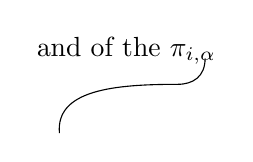
\begin{tikzpicture}[x=1cm,y=1cm]
\node at (.05,.45) {and of the $\pi_{i,\alpha}$};
\draw (-.8,-.6) .. controls (-.85,-.05) and (-.1,.02) .. (.7,.02) .. controls (.9,.02) and (1.05,.12) .. (1.05,.35);
\end{tikzpicture}}} by the formulas $(6.14)$.
\mspage{15}
